\documentclass[border=10pt]{standalone}
\usepackage{tikz}
\usetikzlibrary{positioning}

% --- Anthropic Color Definitions ---
% Primary
\definecolor{slate}{HTML}{141413}
\definecolor{ivory}{HTML}{FAF9F5}
\definecolor{clay}{HTML}{D97757}

% Secondary
\definecolor{sky}{HTML}{6A9BCC}
\definecolor{olive}{HTML}{788C5D}
\definecolor{fig}{HTML}{C46686}
\definecolor{cactus}{HTML}{BCD1CA}
\definecolor{oat}{HTML}{E3DACC}

% PRETTY_CYCLE
\definecolor{darkorange}{HTML}{B86046}
\definecolor{grey}{HTML}{656565}
\definecolor{darkblue}{HTML}{40668C}
\definecolor{kraft}{HTML}{D19B75}
\definecolor{lightpurple}{HTML}{8778AB}
\definecolor{darkpurple}{HTML}{4A366F}

% Grayscale
\definecolor{gray700}{HTML}{3D3D3A}
\definecolor{gray400}{HTML}{B0AEA5}
\definecolor{gray200}{HTML}{E8E6DC}

% --- Node Styles ---
\tikzset{
  anthropic node/.style={
    draw=gray400,
    fill=ivory,
    text=slate,
    rounded corners=4pt,
    inner sep=10pt,
    font=\sffamily,
  },
  input node/.style={
    anthropic node,
    circle,
    minimum size=1cm,
    inner sep=0pt,
    fill=sky!20,
    draw=sky,
  },
  hidden node/.style={
    anthropic node,
    circle,
    minimum size=1cm,
    inner sep=0pt,
    fill=clay!15,
    draw=clay,
  },
  output node/.style={
    anthropic node,
    circle,
    minimum size=1cm,
    inner sep=0pt,
    fill=olive!20,
    draw=olive,
  },
  layer label/.style={
    font=\sffamily\bfseries,
    text=slate,
  },
}

\begin{document}
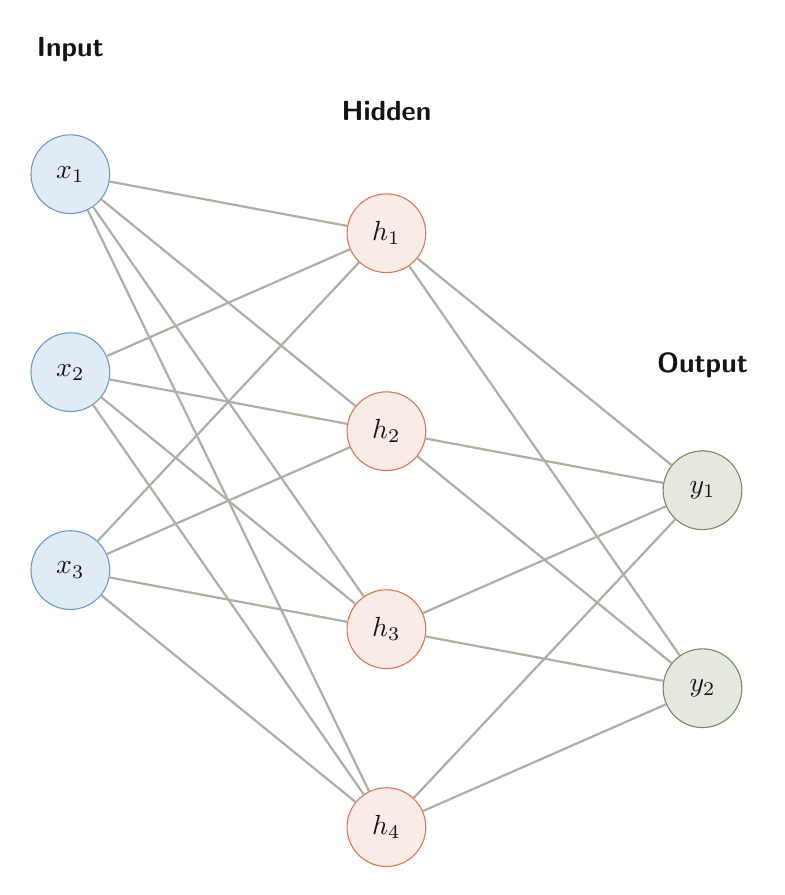
\begin{tikzpicture}[node distance=1.5cm and 3cm]

  % --- Input Layer (3 nodes) ---
  \node[input node] (i1) {$x_1$};
  \node[input node, below=1.5cm of i1] (i2) {$x_2$};
  \node[input node, below=1.5cm of i2] (i3) {$x_3$};

  % --- Hidden Layer (4 nodes) ---
  \node[hidden node, right=3cm of i1, yshift=-0.75cm] (h1) {$h_1$};
  \node[hidden node, below=1.5cm of h1] (h2) {$h_2$};
  \node[hidden node, below=1.5cm of h2] (h3) {$h_3$};
  \node[hidden node, below=1.5cm of h3] (h4) {$h_4$};

  % --- Output Layer (2 nodes) ---
  \node[output node, right=3cm of h2, yshift=-0.75cm] (o1) {$y_1$};
  \node[output node, below=1.5cm of o1] (o2) {$y_2$};

  % --- Connections: Input -> Hidden ---
  \foreach \i in {1,2,3} {
    \foreach \h in {1,2,3,4} {
      \draw[gray400, thick] (i\i) -- (h\h);
    }
  }

  % --- Connections: Hidden -> Output ---
  \foreach \h in {1,2,3,4} {
    \foreach \o in {1,2} {
      \draw[gray400, thick] (h\h) -- (o\o);
    }
  }

  % --- Layer Labels ---
  \node[layer label, above=0.8cm of i1] {Input};
  \node[layer label, above=0.8cm of h1] {Hidden};
  \node[layer label, above=0.8cm of o1] {Output};

\end{tikzpicture}
\end{document}
